\section{View}
\subsection{Klassendiagramm}
\begin{center}
	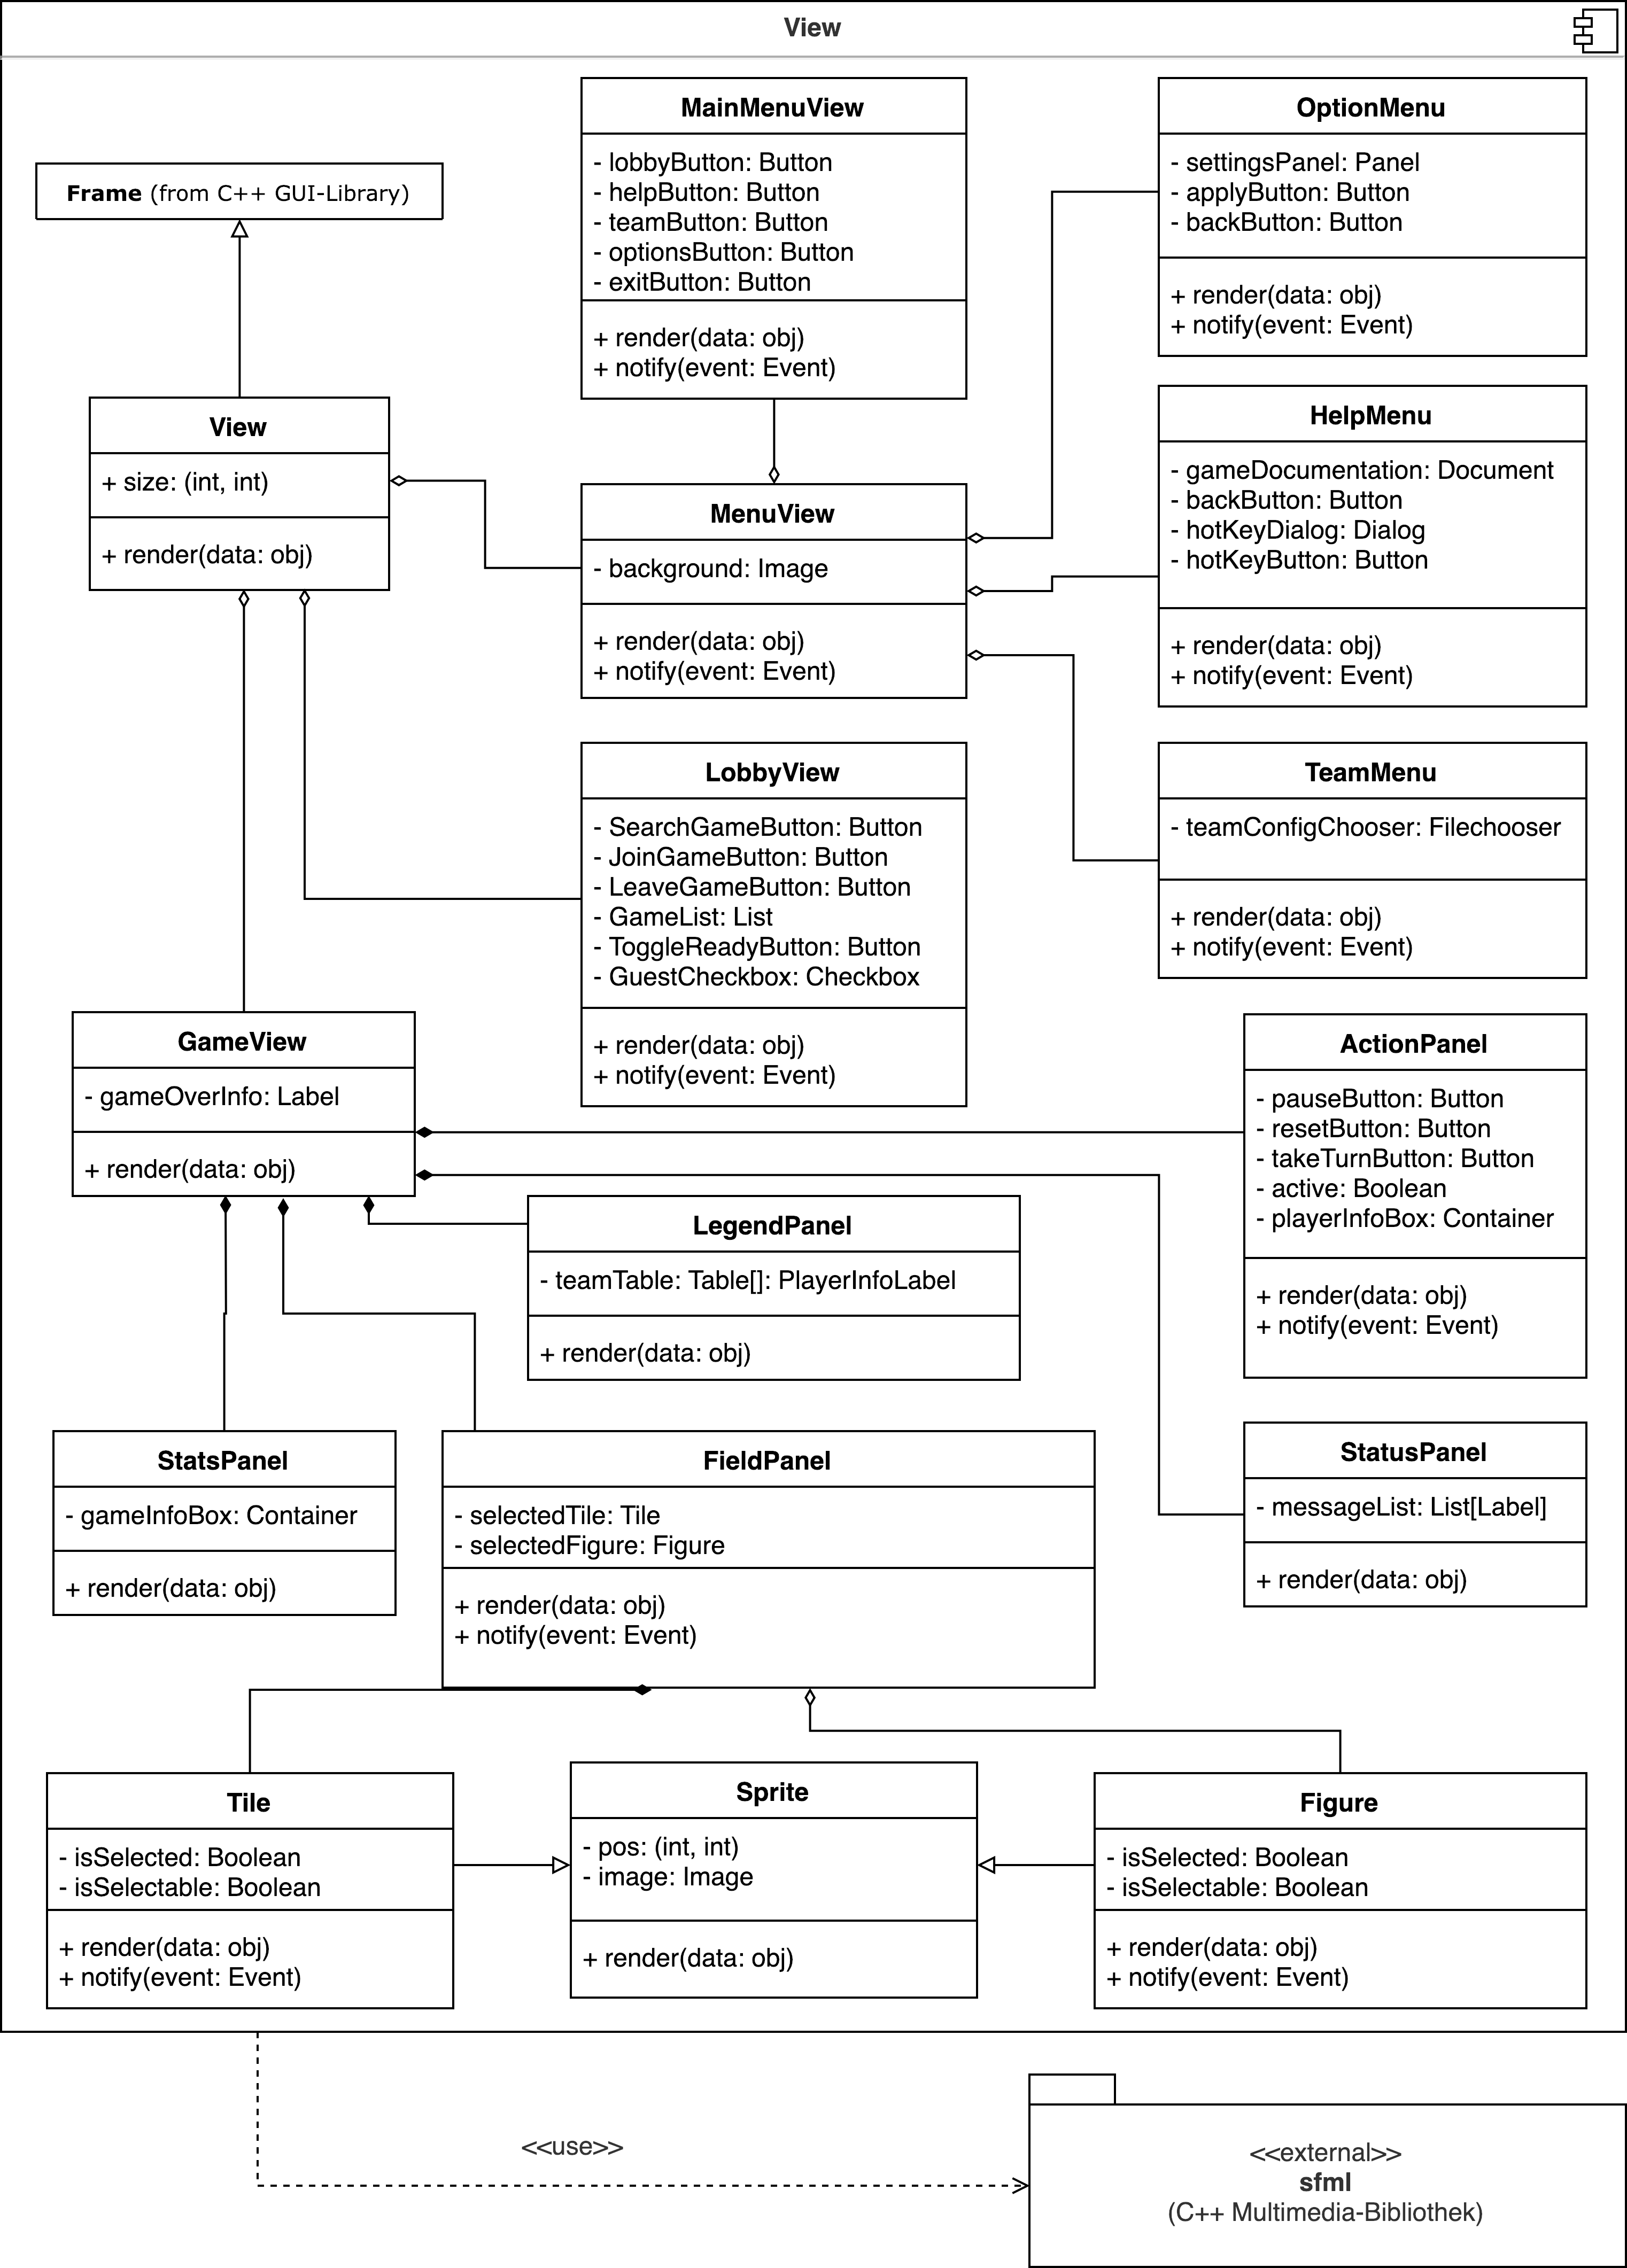
\includegraphics[width=14cm]{images/klassendiagramm_view_extended}
\end{center}

\subsection{Beschreibung}
	Im Folgenden werden die eingetragenen Methoden erklärt. Da in der gesamten Komponente der View auf eine externe Bibliothek zurückgegriffen werden wird, ist dies auf dem Diagramm entsprechend angedeutet.
\begin{description}
	\item[render (Methode)]
		Die render-Methode von Klassen in der View rendert bei jedem Aufruf die enthaltenen Objekte auf dem Anwendungsfenster.
	\item[notify (Methode)]
		Die notify-Methode von Klassen in der View leitet die entsprechenden Event der Elemente in der GUI an den Controller weiter.
	
	\item[sfml (externe Bibliothek)]
		Bei sfml handelt es sich um eine portable API für C++. Insgesamt stellt es eine komplette Multimedia-Bibliothek dar. Hier wird es als Fenster-Manager und GUI-Bibliothek sowie zur Darstellung von 2D-Grafik-Objekten und ggf. zum Abspielen von Musik verwendet.
		Da eine endgültige Festlegung auf diese Bibliothek noch nicht stattgefunden hat, ist ihre Verwendung auf dem Klassendiagramm nur angedeutet und noch nicht fest eingearbeitet. Die Bezeichnungen der entsprechenden Klassen im Diagramm sind daher möglichst allgemein gehalten.
\end{description}


\subsection{Zuordnung der funktionalen Anforderungen}
Die Funktionalen Anforderungen werden den Methoden folgendermaßen zugeteilt:
\begin{center}
	\begin{tabular}{|l|l|}
		\hline
		\textbf{Funktionale Anforderungen} & \textbf{Methoden}\\\hline
		FA60 & MainMenuView::render\\
		FA61& LobbyView::render\\\hline
		FA62 & GameView::render\\\hline
		FA63 & TeamMenu::render, TeamMenu::notify\\\hline
		FA64 & GameView::render\\\hline
		FA65 & HelpMenu::render\\\hline
		FA66 & GameView::render\\\hline
		
	\end{tabular}
\end{center}
